\documentclass[10pt, aspectratio=169]{beamer}

\usetheme{metropolis}
\metroset{progressbar=frametitle}
\metroset{block=fill}

% ============================================================
% UNSW Color Scheme
% ============================================================
\definecolor{UNSWDarkBlue}{HTML}{000F2B}
\definecolor{UNSWYellow}{HTML}{FFD200}
\definecolor{UNSWRed}{HTML}{E63E30}
\definecolor{UNSWLightGray}{HTML}{F0F0F0}
\definecolor{UNSWGreen}{HTML}{00843D}

\setbeamercolor{frametitle}{bg=UNSWYellow, fg=UNSWDarkBlue}
\setbeamercolor{title separator}{fg=UNSWDarkBlue}
\setbeamercolor{progress bar}{fg=UNSWDarkBlue, bg=UNSWDarkBlue!20}
\setbeamercolor{progress bar in head/foot}{fg=UNSWDarkBlue, bg=UNSWDarkBlue!20}
\setbeamercolor{progress bar in section page}{fg=UNSWDarkBlue, bg=UNSWDarkBlue!20}
\setbeamercolor{normal text}{fg=UNSWDarkBlue, bg=white}
\setbeamercolor{alerted text}{fg=UNSWRed}
\setbeamercolor{palette primary}{bg=UNSWDarkBlue, fg=white}
\setbeamercolor{block title}{bg=UNSWDarkBlue, fg=white}
\setbeamercolor{block body}{bg=UNSWLightGray, fg=UNSWDarkBlue}
\setbeamercolor{structure}{fg=UNSWDarkBlue}
\setbeamercolor{item}{fg=UNSWDarkBlue}

\usepackage{booktabs}
\usepackage{graphicx}
\usepackage{amsmath, amssymb}
\usepackage{hyperref}
\usepackage{tikz}
\usetikzlibrary{shapes.geometric, arrows.meta, positioning, calc, fit}
\usepackage{appendixnumberbeamer}
\usepackage{pifont}
\usepackage{colortbl}
\usepackage[backend=bibtex, style=numeric, maxnames=2, sorting=none]{biblatex}
\addbibresource{references.bib}

\newcommand{\cmark}{{\color{UNSWGreen}\ding{51}}}
\newcommand{\xmark}{{\color{UNSWRed}\ding{55}}}
\setlength{\parskip}{0pt}

% ============================================================
% Metadata
% ============================================================
\title{Multi-Task Financial NLP: Stance \& Sentiment Classification}
\subtitle{COMP6713 --- Natural Language Processing --- 2026 T1}
\author{Louis Nguyen \and Quoc Dat Bui \and Nam Khanh Tran \and Quang Minh Phan}
\institute{UNSW School of Computer Science and Engineering}
\date{\today}

\begin{document}

% ============================================================
% 1. Title
% ============================================================
\begin{frame}
    \titlepage
\end{frame}

% ============================================================
% 2. Problem + Datasets
% ============================================================
\begin{frame}{Problem \& Datasets}
    \begin{columns}[T]
        \begin{column}{0.5\textwidth}
            \textbf{Two 3-class classification tasks:}
            \begin{itemize}\setlength{\itemsep}{2pt}
                \item \textbf{Stance} (FOMC monetary policy)\\ \{hawkish, dovish, neutral\}
                \item \textbf{Sentiment} (financial news)\\ \{positive, negative, neutral\}
            \end{itemize}
            \vspace{0.5em}
            \textbf{Why it matters:}
            \begin{itemize}\setlength{\itemsep}{2pt}
                \item Central-bank stance moves markets
                \item Shared financial vocabulary, different tasks $\Rightarrow$ natural MTL setup
            \end{itemize}
        \end{column}
        \begin{column}{0.5\textwidth}
            \textbf{Datasets (70/10/20 stratified, seed 42):}\\[0.4em]
            {\footnotesize
            \begin{tabular}{lccc}
                \toprule
                & Total & Train & Test \\
                \midrule
                FOMC~\cite{shah2023trillion}       & 2{,}480 & 1{,}736 & 496 \\
                FPB all-agree~\cite{malo2014good}  & 2{,}264 & 1{,}584 & 453 \\
                \bottomrule
            \end{tabular}}
            \vspace{0.5em}
            \begin{itemize}\setlength{\itemsep}{2pt}
                \item FPB test: 61/278/114 (\textbf{neu-dominant})
                \item FOMC test: 130/121/245 (balanced-ish)
                \item LM lexicon~\cite{loughran2011liability} for rule-based baseline
            \end{itemize}
        \end{column}
    \end{columns}
\end{frame}

% ============================================================
% 3. Pipeline + Fine-tuning
% ============================================================
\begin{frame}{Methodology: 6-Stage Model Ladder}
    \vspace{-0.3em}
    \begin{center}
    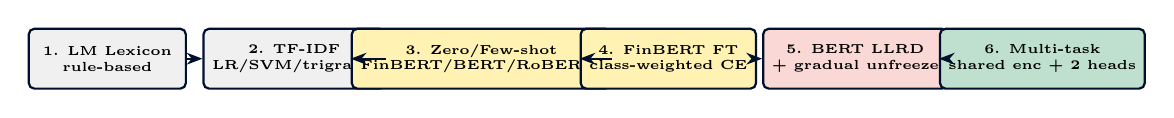
\begin{tikzpicture}[
        box/.style={draw=UNSWDarkBlue, rounded corners=2pt, minimum width=2.1cm, minimum height=0.8cm, align=center, font=\tiny\bfseries, line width=0.8pt},
        arr/.style={-{Stealth[length=2mm]}, line width=0.8pt, UNSWDarkBlue},
        scale=0.95, transform shape
    ]
        \node[box, fill=UNSWLightGray]  (s1) at (0, 0) {1. LM Lexicon\\{\tiny rule-based}};
        \node[box, fill=UNSWLightGray]  (s2) at (2.5, 0) {2. TF-IDF\\{\tiny LR/SVM/trigrams}};
        \node[box, fill=UNSWYellow!30]  (s3) at (5.0, 0) {3. Zero/Few-shot\\{\tiny FinBERT/BERT/RoBERTa}};
        \node[box, fill=UNSWYellow!30]  (s4) at (7.5, 0) {4. FinBERT FT\\{\tiny class-weighted CE}};
        \node[box, fill=UNSWRed!20]     (s5) at (10.0, 0) {5. BERT LLRD\\{\tiny + gradual unfreeze}};
        \node[box, fill=UNSWGreen!25]   (s6) at (12.5, 0) {6. Multi-task\\{\tiny shared enc + 2 heads}};
        \draw[arr] (s1) -- (s2); \draw[arr] (s2) -- (s3); \draw[arr] (s3) -- (s4);
        \draw[arr] (s4) -- (s5); \draw[arr] (s5) -- (s6);
    \end{tikzpicture}
    \end{center}
    \vspace{0.3em}
    \begin{columns}[T]
        \begin{column}{0.5\textwidth}
            \textbf{FinBERT fine-tune}
            \begin{itemize}\setlength{\itemsep}{0pt}
                \item AdamW, lr $2\mathrm{e}{-5}$, 5 epochs, batch 32
                \item Class weights $(1.272, 1.365, 0.675)$ for stance
                \item Linear warmup (10\%) $\rightarrow$ linear decay
            \end{itemize}
        \end{column}
        \begin{column}{0.5\textwidth}
            \textbf{BERT-base LLRD + gradual unfreezing}~\cite{howard2018ulmfit,sun2019finetune}
            \begin{itemize}\setlength{\itemsep}{0pt}
                \item $\eta_d = 2\mathrm{e}{-5} \cdot 0.9^{\,d}$ per layer group
                \item Unfreeze 1 layer group per epoch (10 epochs)
                \item Label smoothing $\varepsilon = 0.1$
            \end{itemize}
        \end{column}
    \end{columns}
\end{frame}

% ============================================================
% 4. Multi-task Architecture (KEY)
% ============================================================
\begin{frame}{Multi-task FinBERT Architecture (main contribution)}
    \begin{columns}[T]
        \begin{column}{0.55\textwidth}
            \centering
            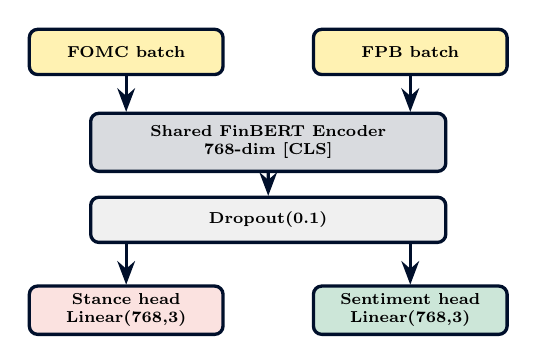
\begin{tikzpicture}[
                box/.style={draw=UNSWDarkBlue, rounded corners=3pt, minimum width=3.0cm, minimum height=0.7cm, align=center, font=\scriptsize\bfseries, line width=1.2pt},
                arr/.style={-{Stealth[length=3mm]}, line width=1.2pt, UNSWDarkBlue},
                scale=0.82, transform shape
            ]
                \node[box, fill=UNSWYellow!30] (inpA) at (-2.2, 4.0) {FOMC batch};
                \node[box, fill=UNSWYellow!30] (inpB) at (2.2, 4.0) {FPB batch};
                \node[box, fill=UNSWDarkBlue!15, minimum width=5.5cm, minimum height=0.9cm] (enc) at (0, 2.6) {\textbf{Shared FinBERT Encoder}\\{\scriptsize 768-dim [CLS]}};
                \node[box, fill=UNSWLightGray, minimum width=5.5cm] (drop) at (0, 1.4) {Dropout(0.1)};
                \node[box, fill=UNSWRed!15] (h1) at (-2.2, 0.0) {Stance head\\{\scriptsize Linear(768,3)}};
                \node[box, fill=UNSWGreen!20] (h2) at (2.2, 0.0) {Sentiment head\\{\scriptsize Linear(768,3)}};
                \draw[arr] (inpA.south) -- (enc.north -| inpA.south);
                \draw[arr] (inpB.south) -- (enc.north -| inpB.south);
                \draw[arr] (enc) -- (drop);
                \draw[arr] (drop.south -| h1.north) -- (h1.north);
                \draw[arr] (drop.south -| h2.north) -- (h2.north);
            \end{tikzpicture}
        \end{column}
        \begin{column}{0.42\textwidth}
            \textbf{Training}~\cite{liu2019mt-dnn}:
            \begin{itemize}\setlength{\itemsep}{2pt}
                \item \textbf{Alternating batches}: one FOMC, then one FPB; active task's head receives gradient, inactive receives zero.
                \item AdamW lr $2\mathrm{e}{-5}$, 8 epochs, batch 32.
                \item Per-task CE (class-weighted for stance).
                \item Best checkpoint by \textit{average} validation macro-F1.
            \end{itemize}
            \vspace{0.3em}
            {\small Shared encoder $\Rightarrow$ each task regularises the other $\Rightarrow$ free data-augmentation effect.}
        \end{column}
    \end{columns}
\end{frame}

% ============================================================
% 5. Headline Results
% ============================================================
\begin{frame}[t]{Results --- All 12 Systems}
    \vspace{-0.4em}
    \centering
    {\footnotesize
    \begin{tabular}{lcccc}
        \toprule
        \textbf{Model} & \textbf{Sent.\ Acc} & \textbf{Sent.\ F1} & \textbf{Stance Acc} & \textbf{Stance F1} \\
        \midrule
        LM Lexicon (rule-based)             & 0.6932 & 0.5315 & 0.4153 & 0.3885 \\
        TF-IDF + LR                         & 0.8720 & 0.8232 & 0.6089 & 0.5873 \\
        TF-IDF + SVM (LinearSVC)            & 0.8940 & 0.8534 & 0.6331 & 0.6061 \\
        TF-IDF (trigrams) + LR              & 0.8786 & 0.8310 & 0.6109 & 0.5914 \\
        TF-IDF + LM Lexicon (hybrid)        & 0.8543 & 0.8050 & 0.6109 & 0.5863 \\
        \midrule
        FinBERT zero-shot (native)          & 0.9735 & 0.9650 & 0.4980 & 0.4874 \\
        FinBERT few-shot (k=16 probe)       & 0.9779 & 0.9670 & 0.4859 & 0.4534 \\
        BERT-base few-shot (k=16)           & 0.7417 & 0.6500 & 0.3851 & 0.3744 \\
        RoBERTa-base few-shot (k=16)        & 0.7682 & 0.6722 & 0.3730 & 0.3600 \\
        \midrule
        FinBERT (fine-tuned)                & 0.9669 & 0.9459 & 0.6371 & 0.6194 \\
        \rowcolor{UNSWYellow!30}
        BERT-base LLRD + Gradual UF         & 0.9757 & \textbf{0.9670} & \textbf{0.6512} & \textbf{0.6383} \\
        \rowcolor{UNSWYellow!30}
        \textbf{Multi-task FinBERT}         & \textbf{0.9779} & \textbf{0.9666} & 0.6492 & \textbf{0.6384} \\
        \bottomrule
    \end{tabular}}
    \vspace{0.4em}
    {\small \textbf{Top-2 tied}: Multi-task FinBERT vs BERT-LLRD within $\pm 0.1$ pp.
    Multi-task \textbf{beats} single-task FinBERT by \textbf{+2.07 pp} sentiment F1 and \textbf{+1.90 pp} stance F1.}
\end{frame}

% ============================================================
% 6. Analysis / Key Findings
% ============================================================
\begin{frame}{Key Findings \& Error Analysis}
    \begin{columns}[T]
        \begin{column}{0.55\textwidth}
            \textbf{Findings}:
            \begin{enumerate}\setlength{\itemsep}{2pt}
                \item \textbf{Sentiment is near-solved} (F1 $\approx 0.97$); \textbf{stance is hard} (F1 $\approx 0.64$) --- 33 pp task-difficulty gap.
                \item \textbf{Domain pretraining dominates in low-data}: at $k=16$, FinBERT beats BERT/RoBERTa by $\approx 30$ pp sentiment F1.
                \item \textbf{Multi-task helps stance more} ($+1.90$ pp) than sentiment ($+2.07$ pp on a near-saturated task).
                \item \textbf{Careful fine-tuning rivals domain pretraining}: BERT LLRD + gradual unfreeze ties multi-task FinBERT.
            \end{enumerate}
        \end{column}
        \begin{column}{0.43\textwidth}
            \textbf{Error patterns (Multi-task FinBERT)}:\\[0.3em]
            {\footnotesize
            \begin{tabular}{lc}
                \toprule
                Per-class F1 & score \\
                \midrule
                Sent.\ neutral   & 0.9928 \\
                Sent.\ positive  & 0.9569 \\
                Sent.\ negative  & 0.9500 \\
                \midrule
                Stance neutral   & 0.7109 \\
                Stance dovish    & 0.6174 \\
                Stance \textbf{hawkish}   & \textbf{0.5869} \\
                \bottomrule
            \end{tabular}}
            \vspace{0.4em}
            {\footnotesize \textbf{Hawkish} weakest: smallest train set (424) \& most hedged language (``some participants noted'').}
        \end{column}
    \end{columns}
\end{frame}

% ============================================================
% 7. Deployment + Demo
% ============================================================
\begin{frame}{Deployment \& Live Demo}
    \begin{columns}[T]
        \begin{column}{0.48\textwidth}
            \textbf{Three interfaces}:
            \begin{itemize}\setlength{\itemsep}{3pt}
                \item \textbf{CLI} \texttt{cli.py}:\\
                      {\small \texttt{--text} / \texttt{--file} / interactive}
                \item \textbf{Gradio demo} \texttt{demo.py}:\\
                      {\small web UI at \texttt{localhost:7860}}
                \item \textbf{HuggingFace Hub}: 5 public repos\\
                      {\scriptsize
                      \texttt{Louisnguyen/\allowbreak multitask-finbert-financial}\\
                      \texttt{Louisnguyen/\allowbreak finbert-financial-\{stance,sentiment\}}\\
                      \texttt{Louisnguyen/\allowbreak bert-llrd-financial-\{stance,sentiment\}}}
            \end{itemize}
        \end{column}
        \begin{column}{0.48\textwidth}
            \centering
            \begin{block}{\centering Live Demo}
                \centering
                \vspace{0.3em}
                Switching to Gradio at \texttt{http://localhost:7860}
                \vspace{0.3em}
            \end{block}
            \vspace{0.5em}
            \textbf{Example inputs}:
            \begin{itemize}\setlength{\itemsep}{1pt}
                \item ``The Fed signaled further rate hikes ahead.''
                \item ``Operating profit rose sharply in Q3.''
                \item ``Some participants observed inflation pressures have eased.''
            \end{itemize}
        \end{column}
    \end{columns}
\end{frame}

% ============================================================
% 8. Summary
% ============================================================
\begin{frame}{Summary \& Takeaways}
    \begin{block}{Problem}
        Stance (FOMC) + sentiment (FPB) classification --- 2,480 + 2,264 sentences.
    \end{block}
    \begin{block}{Approach}
        12-system ladder: lexicon $\rightarrow$ TF-IDF $\rightarrow$ zero/few-shot $\rightarrow$ fine-tune $\rightarrow$ \textbf{LLRD + gradual unfreeze} $\rightarrow$ \textbf{multi-task FinBERT}.
    \end{block}
    \begin{block}{Headline result}
        Multi-task FinBERT: \textbf{97.79\%} / \textbf{0.9666} sentiment, \textbf{64.92\%} / \textbf{0.6384} stance. Multi-task beats single-task FinBERT by \textbf{+2.07 pp} sent, \textbf{+1.90 pp} stance.
    \end{block}
    \begin{block}{Lesson}
        Domain pretraining \textbf{and} careful fine-tuning recipes are \textit{substitutes}, not complements --- BERT-LLRD ties Multi-task FinBERT.
    \end{block}
    \vspace{0.3em}
    \centering \Large \textbf{Q\&A}
\end{frame}

% ============================================================
% References (backup, not counted in 8)
% ============================================================
\begin{frame}[allowframebreaks]{References}
    \printbibliography[heading=none]
\end{frame}

\end{document}
